\subsubsection{Two options to start Java \gdauts{}}
\gdhelpid{autConfigSettingWizardPagePageContextId}{Configuring an AUT}
\gdhelpid{autSettingWizardPagePageContextId}{Defining an AUT}

\app{} offers two options to start your Java \gdaut{} for testing:

\begin{description}
\item [Via an \gdaut{} configuration:]{This option means that you create an \gdaut{} configuration in your \gdproject{}, and the \gdaut{} is started by \app{} \bxpref{TasksConfigureJavaAUT}.}
\item [Using the \bxname{autrun} command:]{This option lets you start an \gdaut{} without creating a configuration. Certain start parameters are required for the \gdaut{} so that \app{} can locate it \bxpref{autrun}.}
\end{description}


\subsubsection{Configuring a Java \gdaut{} to be started by \app{}}
\index{Add!AUT Configuration}
\index{AUT Configuration!Add}
\index{Edit!AUT Configuration}
\index{AUT Configuration!Edit}
\index{Classpath}
\index{Working Directory}
\index{Classname}
\index{CmdLineParameter}
\index{Environment}
\index{AUT!Configuration}
\index{Configuration!AUT}
\index{Activation}
\index{Application activation}
\index{AUT ID}
\label{TasksConfigureJavaAUT}

The \gdaut{} configuration dialog for Java has three different levels of detail: basic, advanced and expert. 

See the sections below for information on the different levels. 

\subsubsection{Basic Java \gdaut{} configuration}

You can use the basic setting (\bxfigref{autconfigbasic}) to configure your \gdaut{} if it can be started by an executable file (e.g. .bat, .exe, .cmd, .sh etc.) and if it is written in Java 1.5 or above, and you are using a Java Standard Edition JRE. 
\bxwarn{If you are testing RCP or GEF \gdauts{}, there are certain specific steps you need to take to configure them. See the sections on RCP testing \bxpref{rcpaut}, GEF testing \bxpref{geftest} for details. }

\begin{figure}[h]
\begin{center}
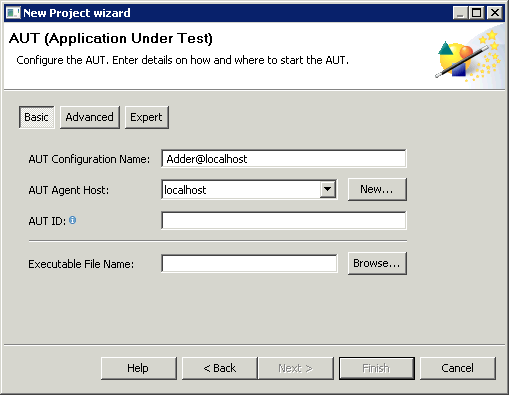
\includegraphics{Tasks/AUTs/PS/autconfigwindow_basic}
\caption{\gdaut configuration window: basic}
\label{autconfigbasic}
\end{center}
\end{figure}

\begin{enumerate}
\item A suggested name for this \gdaut{} configuration is generated automatically based on your \gdaut{} name and the default \gdagent{} host. You can change this name if you wish. 
\item The default \gdagent host is also automatically selected. You can select a new \gdagent{} from the combo box or add a new one by clicking \bxcaption{New}. For more information on adding and editing an \gdagent{}, see the section later \bxpref{TasksPrefsAgent}.

\item Enter the executable file name in the \bxname{Executable File Name} field. This path can be relative if you define a working directory \bxpref{AdvancedAUTConfig}).
\item Enter the \gdaut{} ID that will be given to this \gdaut{} when it is started.  
\end{enumerate}
For information on the advanced properties for the \gdaut{} configuration, see the next section \bxpref{AdvancedAUTConfig}. 


\subsubsection{Advanced \gdaut{} configuration}
\label{AdvancedAUTConfig}

You can use the advanced dialog (\bxfigref{autconfigadvanced}) if your \gdaut{} is a Java JAR which can be started with a double click, or if your application can be started using the class name and the classpaths to your \gdaut{}.  The advanced configuration dialog also lets you create a working directory for your \gdaut{}, and add command-line arguments needed to start the \gdaut{}. You can select a JRE executable and, for SWT/RCP \gdauts{}, a keyboard layout.

\begin{figure}[h]
\begin{center}
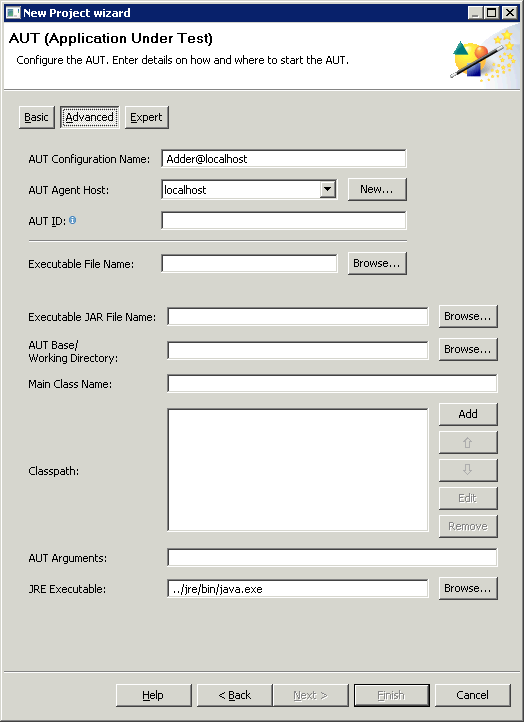
\includegraphics{Tasks/AUTs/PS/autconfigwindowadvanced}
\caption{\gdaut configuration window: advanced}
\label{autconfigadvanced}
\end{center}
\end{figure}

\begin{enumerate}
\item Enter the JAR path (directory and file
  name) into the \bxname{Executable JAR File Name} field.  

This path can be relative (if you define a working directory), or absolute. This JAR file must contain a manifest file which contains the main class and the classpath. 

\item You can optionally create a working directory to store files in. The server directory of the \app{} installation is selected as default. To create a working directory elsewhere, browse to and select the location. 

The working directory is the root directory for any classpaths, classnames, JAR files and JRE binaries. If you create a working directory, you can enter the paths to these items using a relative path, with the working directory as the root. For more information on relative paths, read the section in the reference manual \bxextref{\gdrefman}{ref,relativepath}. 

\item If your \gdaut{} must be started with the class name, add the main class name and the classpaths into their relative fields. The paths can be relative (if you have defined a working directory), or absolute. 
\bxtipp{Add all the necessary files and directories to start the \gdaut{}. }
\item Enter any necessary command-line arguments for the \gdaut{} in the
 \bxname{AUT Arguments} field. 
\item Browse to a JRE executable or add a new one by clicking \bxcaption{New}. 
The Java version used must be 1.4 or later. 

Java is installed with \app{}. You can find the Java file in:\\
\bxmenu{\app{}}{jre}{bin}.
Use java.exe if you want to use a console, use javaw.exe if you do not want a console. 
\item For SWT and RCP \gdauts{}, select which keyboard layout is used on the machine on which the \gdaut{} will run. 
g
\bxtipp{The keyboard layout is not the actual keyboard attached to the computer, but is based on the regional language settings for the operating system.}

\app{} supports English (US) and German (DE) keyboard layouts out-of-the box. If you want to use a different keyboard layout, see the reference manual for information on creating keyboard layouts \bxextref{\gdrefman}{ref,keyboardlayout}. 
\end{enumerate}
For information on the expert properties for the \gdaut{} configuration, see the next section \bxpref{ExpertAUTConfig}. 

\subsubsection{Expert \gdaut{} configuration}
\label{ExpertAUTConfig}
You can use the expert dialog (\bxfigref{autconfigexpert}) to configure more detailed information about how the \gdaut{} should be started. 

\begin{figure}[h]
\begin{center}
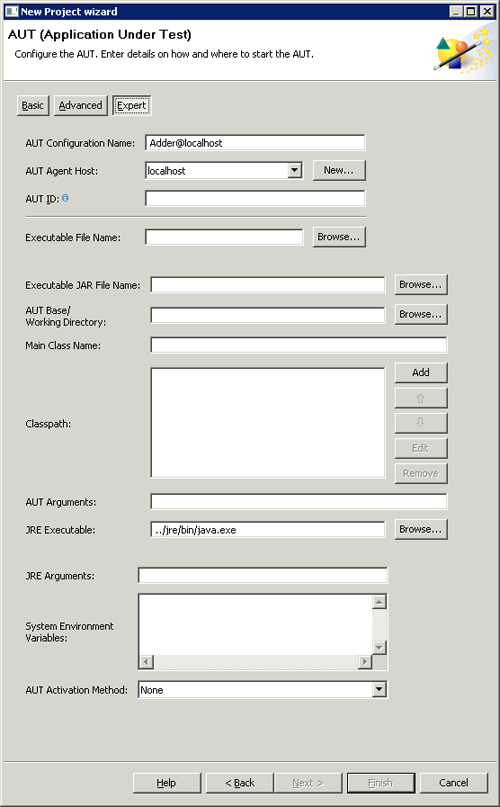
\includegraphics{Tasks/AUTs/PS/autconfigwindow_expert}
\caption{\gdaut configuration window: expert}
\label{autconfigexpert}
\end{center}
\end{figure}

\begin{enumerate}
\item Add any additional desired \bxname{JRE Arguments}. 
\item Enter any required \bxname{System Environment Variables}, in the
format \bxcaption{<VARNAME>=<value>}, i.e. \bxcaption{PATH=C:$\backslash$}. 
Separate each variable with a new line by pressing \bxkey{Enter}.

\bxwarn{Please be advised that ''embedding'' the contents of one
variable into another is not supported at this time by \app{}. That is,
if you have a variable named \texttt{FOO} whose value is
\bxcaption{abc}, and set the value of a second
variable \texttt{BAR} to \bxcaption{\%FOO\%def}, the second variable will
\emph{not} contain \bxcaption{abcdef}, but rather the exact text
\bxcaption{\%FOO\%def}, without evaluating it.}


\item Select an activation method for your \gdaut{}. More information on \gdaut{} activation is available in the previous section \bxpref{TasksAUTActivation}.

\end{enumerate}

\subsubsection{Starting Java \gdauts{} with the \bxname{autrun} command}
\gdhelpid{autSettingWizardPagePageContextId}{Defining an AUT}
\label{autrun}
%% % ----------------------------------------------------------------------
%% \bxversion{0.1}
%% %\bxdocinfo{STATUS}{freigegeben durch}{freigegeben am}{Verteilerliste}
%% \bxdocinfo{DRAFT}{}{}{}
%% % ----------------------------------------------------------------------

%% \end{document}

\index{gdrun command!Define AUT}
\index{Define AUT!gdrun command}

The \bxname{gdrun} command can be used as an alternative to starting your \gdaut{} via \gd{} (i.e. with an \gdaut{} configuration \bxpref{configuringaut}). It can only be used if your \gdaut{} can be started by an executable file (e.g. .bat, .exe, .cmd, .sh etc.) and if it is written in Java 1.5 or above, and you are using a Sun VM. 


\bxwarn{The \bxname{gdrun} command cannot be used for HTML or pure SWT \gdauts{}.}

The command allows you to start your \gdaut{} independently of \gd{}, on a machine where the \gdserver{} is running. The \gd{} client, when connected to this \gdserver{} will then recognize the running \gdaut{} as a testable application. 

To use the \bxname{gdrun} command:
\begin{enumerate}
\item Ensure that the \gdserver{} is installed on the machine where you will be starting the \gdaut{}. 
\item Start your \gdaut{} via the command line by entering \bxshell{gdrun.exe} then the following parameters: 
\begin{table}[h]
\label{gdrunparams}
	\centering
	\begin{tabular}{|l|l|}

	\hline
	\textbf{Detail}&\textbf{Parameter}%&\textbf{Example}
\\
		\hline
                -h 
                &\bxshell{-h}\\
                & Gives parameter help\\
                \hline
                -w, \verb+--+workingdir
                  & \bxshell{-w <directory>}\\
		  &Enter the working directory for the \gdaut{}\\
                  \hline
                  -a, \verb+--+autagenthost
                  & \bxshell{-a <hostname>}\\
		  &Enter the hostname for the \gdserver{}\\
                  \hline
                  -p, \verb+--+autagentport
                  & \bxshell{-p <port number>}\\
		  &Enter the port number for the \gdserver{}\\
                  \hline
                  -swing
                  & \\
		  &If the \gdaut{} is a Swing \gdaut{}\\
                  \hline
                  -rcp
                  & \\
		  &If the \gdaut{} is an RCP \gdaut{}\\
                  \hline
                  -swt
                  & \\
		  &If the \gdaut{} is an SWT \gdaut{}\\
                  \hline
                  -k, \verb+--+kblayout
                  & \bxshell{-k <en\_US>}\\
		  &Enter the keyboard layout for SWT/RCP \gdauts{}\\
                  \hline
                  -i, \verb+--+autid
                  & \bxshell{-i <ID>}\\
		  &Enter the ID to give to this \gdaut{}\\
                  \hline
                  -e, \verb+--+exec
                  & \bxshell{-e <AUT.exe>}\\
		  &Enter the executable file for the \gdaut{}\\
                  \hline
                  -g, \verb+--+generatenames (optional)
                  & \bxshell{-g <true/false>}\\
		  &For RCP \gdauts{}, enter whether \\& to generate technical names.                  \bxpref{Defineaut}\\
                  \hline
                 
	\end{tabular}
	\caption{Parameters for gdrun command}
	\label{paramscmd}
\end{table}
\end{enumerate}

\subsubsection{Creating an \gdaut{} definition from a running \gdaut{}}
\label{createAUTDef}
Once you have started an \gdaut{} using the \bxname{gdrun} command, you can automatically generate an \gdaut{} definition \bxpref{Defineaut} for this \gdaut{}:

\begin{itemize}
\item In the \gdrunautview{}, select the \gdaut{} you want to define (it will be marked as an unknown \gdaut{} ID).
\item Select:\\
 \bxmenu{Create AUT Definition}{}{}\\
from the context menu.
\item The \gdaut{} definition window will appear. Complete the dialog \bxpref{Defineaut} and click \bxcaption{OK}.
\end{itemize}


